% Options for packages loaded elsewhere
\PassOptionsToPackage{unicode}{hyperref}
\PassOptionsToPackage{hyphens}{url}
%
\documentclass[
  11pt,
]{article}
\usepackage{amsmath,amssymb}
\usepackage{iftex}
\ifPDFTeX
  \usepackage[T1]{fontenc}
  \usepackage[utf8]{inputenc}
  \usepackage{textcomp} % provide euro and other symbols
\else % if luatex or xetex
  \usepackage{unicode-math} % this also loads fontspec
  \defaultfontfeatures{Scale=MatchLowercase}
  \defaultfontfeatures[\rmfamily]{Ligatures=TeX,Scale=1}
\fi
\usepackage{lmodern}
\ifPDFTeX\else
  % xetex/luatex font selection
\fi
% Use upquote if available, for straight quotes in verbatim environments
\IfFileExists{upquote.sty}{\usepackage{upquote}}{}
\IfFileExists{microtype.sty}{% use microtype if available
  \usepackage[]{microtype}
  \UseMicrotypeSet[protrusion]{basicmath} % disable protrusion for tt fonts
}{}
\makeatletter
\@ifundefined{KOMAClassName}{% if non-KOMA class
  \IfFileExists{parskip.sty}{%
    \usepackage{parskip}
  }{% else
    \setlength{\parindent}{0pt}
    \setlength{\parskip}{6pt plus 2pt minus 1pt}}
}{% if KOMA class
  \KOMAoptions{parskip=half}}
\makeatother
\usepackage{xcolor}
\usepackage[top=2.5cm, bottom=2.5cm, left=2.5cm, right=2.5cm]{geometry}
\usepackage{graphicx}
\makeatletter
\def\maxwidth{\ifdim\Gin@nat@width>\linewidth\linewidth\else\Gin@nat@width\fi}
\def\maxheight{\ifdim\Gin@nat@height>\textheight\textheight\else\Gin@nat@height\fi}
\makeatother
% Scale images if necessary, so that they will not overflow the page
% margins by default, and it is still possible to overwrite the defaults
% using explicit options in \includegraphics[width, height, ...]{}
\setkeys{Gin}{width=\maxwidth,height=\maxheight,keepaspectratio}
% Set default figure placement to htbp
\makeatletter
\def\fps@figure{htbp}
\makeatother
\setlength{\emergencystretch}{3em} % prevent overfull lines
\providecommand{\tightlist}{%
  \setlength{\itemsep}{0pt}\setlength{\parskip}{0pt}}
\setcounter{secnumdepth}{5}
\usepackage{graphicx}
\usepackage{amsmath}
\usepackage{booktabs}
\usepackage{caption}
\usepackage{fancyhdr}
\usepackage{ragged2e}
\usepackage{multicol}
\justifying
\pagestyle{fancy}
\fancyhead[L]{Delandre, Garcia, Biocchi, Leteurtre}
\fancyfoot[C]{\thepage}
\usepackage{titlesec}
\titlespacing*{\title}{0pt}{0pt}{0pt}
\titlespacing*{\author}{0pt}{-0.5cm}{0pt}
\titlespacing*{\date}{0pt}{-0.5cm}{0pt}
\titlespacing*{\section}{0pt}{0.5cm}{0pt}
\titlespacing*{\subsection}{0pt}{1cm}{0pt}
\titlespacing*{\subsubsection}{0pt}{0.8cm}{0pt}
\usepackage{etoolbox}
\patchcmd{\maketitle}{\vspace*{2\baselineskip}}{}{}{}
\usepackage{titling}
\setlength{\droptitle}{-1.5cm}
\setlength{\headheight}{12pt}
\setlength{\headsep}{5pt}
\setlength{\parindent}{0pt}
\setlength{\parskip}{1pt}
\usepackage{booktabs}
\usepackage{longtable}
\usepackage{array}
\usepackage{multirow}
\usepackage{wrapfig}
\usepackage{float}
\usepackage{colortbl}
\usepackage{pdflscape}
\usepackage{tabu}
\usepackage{threeparttable}
\usepackage{threeparttablex}
\usepackage[normalem]{ulem}
\usepackage{makecell}
\usepackage{xcolor}
\ifLuaTeX
  \usepackage{selnolig}  % disable illegal ligatures
\fi
\usepackage{bookmark}
\IfFileExists{xurl.sty}{\usepackage{xurl}}{} % add URL line breaks if available
\urlstyle{same}
\hypersetup{
  pdftitle={Predicting Mortgage Yield using Regression Analysis},
  pdfauthor={Group 42},
  hidelinks,
  pdfcreator={LaTeX via pandoc}}

\title{\textbf{Predicting Mortgage Yield using Regression Analysis}}
\author{Group 42}
\date{2025-04-07}

\begin{document}
\maketitle

\section{Introduction}\label{introduction}

The study of A. H. Schaaf, 1966, ``Regional Differences in Mortgage
Financing Costs'', investigates the existence and causes of regional
differences in Mortgage financing costs in the United States. While
these differences in Mortgage Yields were decreasing in the early 20th
century, they suprisingly remained stable after World War II. The paper
explores two main explanations for this phenomenon:\\
\strut \\
\textbf{1.} Differences in investment value due to risk, terms, and
liquidity.\\
\textbf{2.} Market imperfections such as legal barriers and information
gaps.\\

The data used in this study comes from the Federal Home Loan Bank Board,
which contains interest rates and fees in 18 SMSAs (Standard
Metropolitan Statistical Areas). The findings suggest that distance from
major financial centers, risk levels, and local demand for savings
significantly affect Mortgage Yields. However, market structure and
overall savings levels play a lesser important role.

The aim of this report is to analyze the data and develop a predictive
model to predict Mortgage Yield (\texttt{mortYld} in \%) based on 6
explanatory variables:\\
\strut \\
- \textbf{X1:} Loan-to-Mortgage Ratio, in \% → High values indicate low
down payments.\\
- \textbf{X2:} Distance from Boston, in miles → Measures regional
proximity to financial centers.\\
- \textbf{X3:} Savings per New Unit Built, in \$ → Indicator of regional
credit demand.\\
- \textbf{X4:} Savings per Capita, in \$ → Measures local savings levels
(credit supply).\\
- \textbf{X5:} Population Increase, 1950-1960, in \% → Proxy for housing
demand growth.\\
- \textbf{X6:} Percentage of First Mortgages from Inter-Regional Banks,
in \% → Indicator of external financing reliance.

\section{Exploratory Data Analysis
(EDA)}\label{exploratory-data-analysis-eda}

\subsection{Load Data and Libraries}\label{load-data-and-libraries}

\begingroup\fontsize{8}{10}\selectfont

\begin{longtable}[t]{lrrrrrrr}
\caption{\label{tab:unnamed-chunk-1}First few rows of the dataset}\\
\toprule
smsa & mortYld & X1 & X2 & X3 & X4 & X5 & X6\\
\midrule
Los Angeles-Long Bea & 6.17 & 78.1 & 3042 & 91.3 & 1738.1 & 45.5 & 33.1\\
Denver & 6.06 & 77.0 & 1997 & 84.1 & 1110.4 & 51.8 & 21.9\\
San Francisco-Oaklan & 6.04 & 75.7 & 3162 & 129.3 & 1738.1 & 24.0 & 46.0\\
Dallas-Fort Worth & 6.04 & 77.4 & 1821 & 41.2 & 778.4 & 45.7 & 51.3\\
Miami & 6.02 & 77.4 & 1542 & 119.1 & 1136.7 & 88.9 & 18.7\\
\addlinespace
Atlanta & 6.02 & 73.6 & 1074 & 32.3 & 582.9 & 39.9 & 26.6\\
\bottomrule
\end{longtable}
\endgroup{}

Here is a display of the first few rows of the dataset. Each SMSA is
described by its Mortgage Yield (\texttt{mortYld}) as the dependent
variable and six explanatory variables (X1 to X6). All data consist of
numerical values and quick checking confirms that there are no missing
values in any region.

\subsection{Univariate Analysis}\label{univariate-analysis}

\subsubsection{Summary Statistics}\label{summary-statistics}

\begingroup\fontsize{8}{10}\selectfont

\begin{longtable}[t]{llllllll}
\caption{\label{tab:unnamed-chunk-3}Summary Statistics of Variables}\\
\toprule
 & mortYld & X1 & X2 & X3 & X4 & X5 & X6\\
\midrule
 & Min.   :5.280 & Min.   :67.00 & Min.   :   0 & Min.   : 32.3 & Min.   : 582.9 & Min.   : 7.50 & Min.   : 2.00\\
 & 1st Qu.:5.678 & 1st Qu.:70.03 & 1st Qu.: 648 & 1st Qu.: 85.9 & 1st Qu.: 792.9 & 1st Qu.:23.18 & 1st Qu.: 9.55\\
 & Median :5.880 & Median :73.25 & Median :1364 & Median :122.2 & Median :1161.3 & Median :27.35 & Median :18.70\\
 & Mean   :5.841 & Mean   :73.38 & Mean   :1389 & Mean   :159.8 & Mean   :1245.9 & Mean   :33.03 & Mean   :20.95\\
 & 3rd Qu.:6.020 & 3rd Qu.:77.22 & 3rd Qu.:1847 & 3rd Qu.:218.2 & 3rd Qu.:1556.6 & 3rd Qu.:44.10 & 3rd Qu.:30.43\\
\addlinespace
 & Max.   :6.170 & Max.   :78.10 & Max.   :3162 & Max.   :428.2 & Max.   :2582.4 & Max.   :88.90 & Max.   :51.30\\
\bottomrule
\end{longtable}
\endgroup{}

Through this summary, we already observe that Mortgage Yields don't vary
much across regions. Most values are between 5.2\% and 6.2\%, suggesting
relatively stable Mortgage rates.

Loan-to-Mortgage Ratios (X1) are concentrated in between 67\% and
78.1\%, indicating relatively consistent lending practices across
regions. Distance from Boston (X2) has a vast range (0--3162 miles),
highlighting geographical diversity and potential financial access
disparities. Savings per New Unit Built (X3) and Savings per Capita (X4)
are characterized by means bigger than medians, representing
right-skewed distributions, thus suggesting regional imbalances in
credit demand and supply in housing affordability across regions.
Population Increase (X5) from 1950 to 1960 varies widely (7.5--88.9\%),
reflecting differing housing market pressures. Lastly, Percentage of
First Mortgages from Inter-Regional Banks (X6) spans from 2.0\% to
51.3\%, meaning that some areas depend heavily on external financing
while others rely more on local institutions.

\subsubsection{Graphical Representation}\label{graphical-representation}

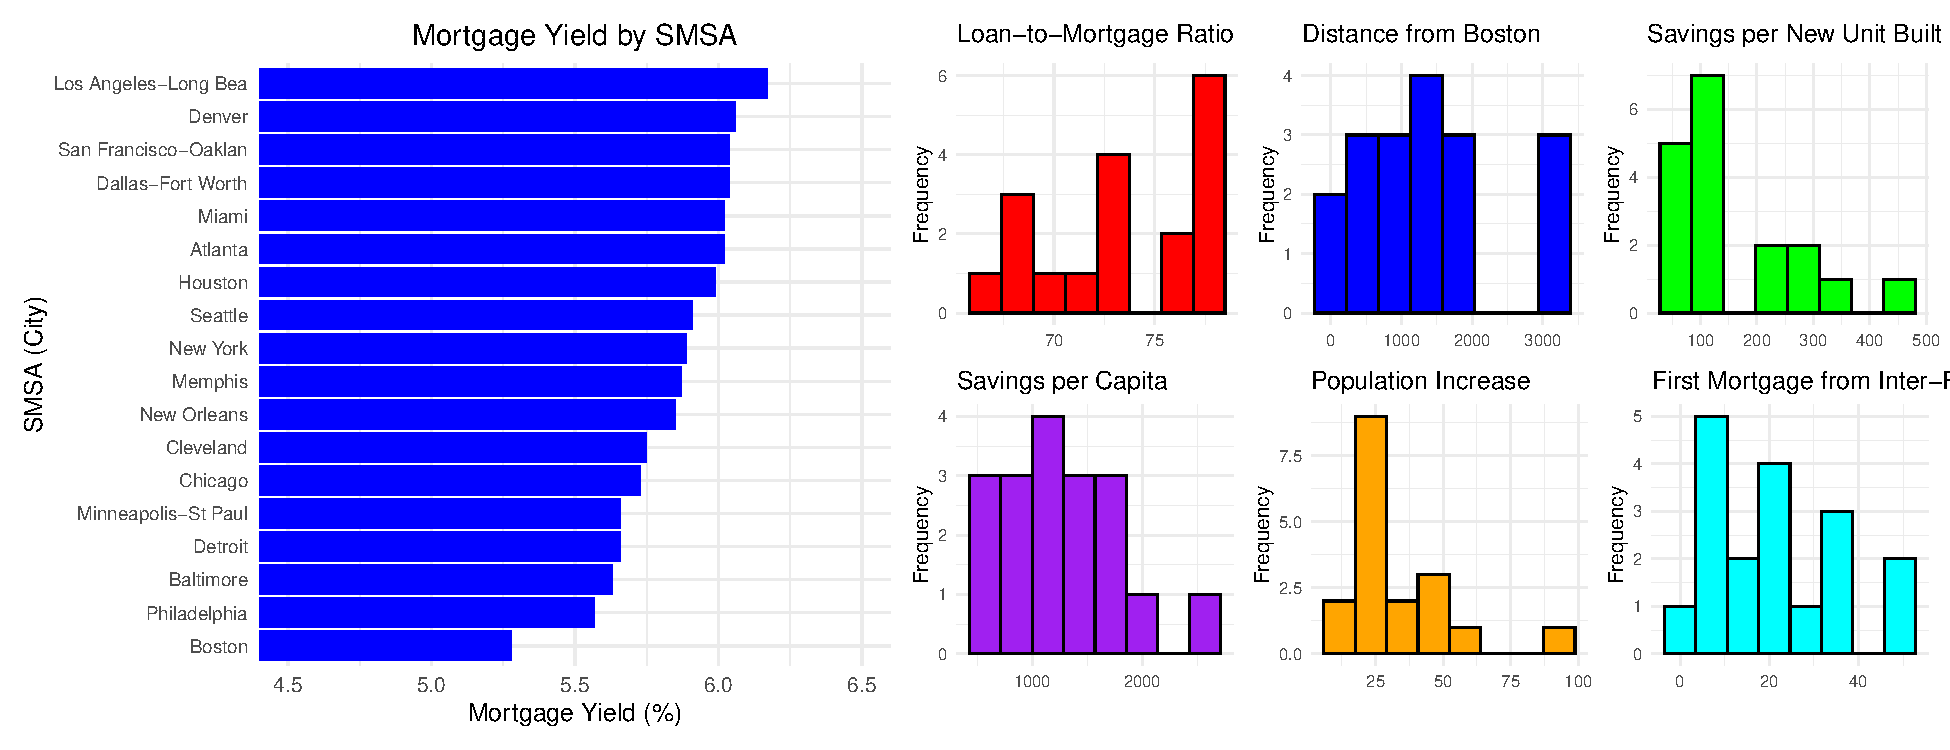
\includegraphics{Figs/unnamed-chunk-4-1.pdf}

With deeper analysis, although the variation across SMSAs is small, we
see that regional differences still exist in Mortgage Yields, possibly
due to economic factors like savings, loan terms, and regional banking
practices. The histograms confirm the distribution of the explanatory
variables:

The Loan-to-Mortgage Ratio (X1) shows low variance with most values
concentrated between 67\% and 80\%, possibly indicating limited
variability across regions. Distance from Boston (X2) displays a wide
and almost homogeneous distribution, reflecting substantial geographic
spread among SMSAs. Savings per New Unit Built (X3) and Savings per
Capita (X4) both exhibit right-skewed distributions, suggesting that a
few cities have notably higher savings levels. Population Increase (X5)
is also highly right-skewed with one major outlier (increase of
\textasciitilde25\%), indicating that most regions had moderate growth,
while a few experienced rapid expansion. Finally, the percentage of
First Mortgages from Inter-Regional Banks (X6) is also right-skewed,
with most cities relying minimally on external financing and a few
showing heavy dependence. Overall, the data suggests regional variation
in housing finance conditions, credit accessibility, and Mortgage market
dynamics.

\subsection{Bivariate Numerical
Analysis}\label{bivariate-numerical-analysis}

\subsubsection{Association Analysis}\label{association-analysis}

\begin{minipage}{0.47\textwidth}
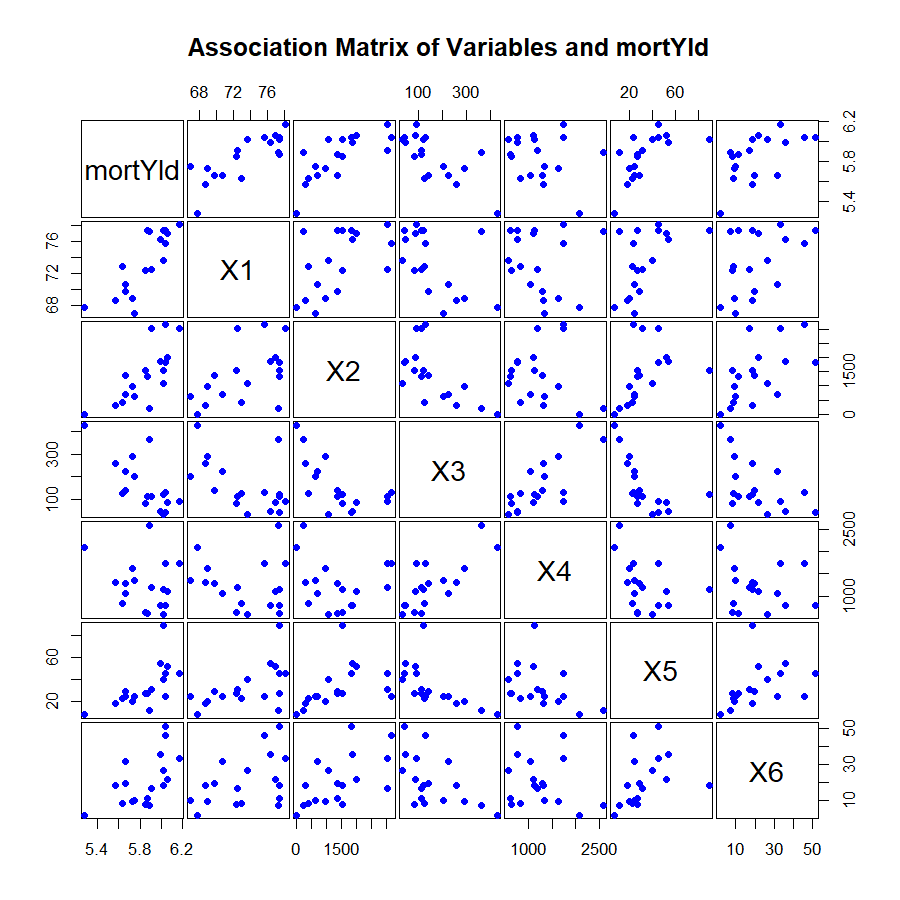
\includegraphics[width=0.85\linewidth]{association_matrix.png}
\end{minipage}
\hfill
\begin{minipage}{0.49\textwidth}
\small
The Association Matrix provides a quick visual assessment of bivariate relationships (how each variable relates to the others and \texttt{mortYld}), of types of associations among predictors (if a relationship looks linear, curved or weak, as well as positive or negative), and of outlier presence. It complements numerical analyses like the correlation matrix and VIF.\\

We can see that most of the plots are random dispersion, while some are linear, and some are curved. \textbf{X3} seems to be positively associated with \textbf{X4} and negatively with \textbf{X5}. \textbf{X2} and \textbf{X3} seem negatively exponentially associated. \textbf{X6} seems to be negatively associated with \textbf{X3}.
\end{minipage}

Let's take a closer look into the Association Matrix, regarding the
relationship between Mortgage Yield (\%) and the explanatory variables
(x-axis), representing the first row in the precedent figure.\\

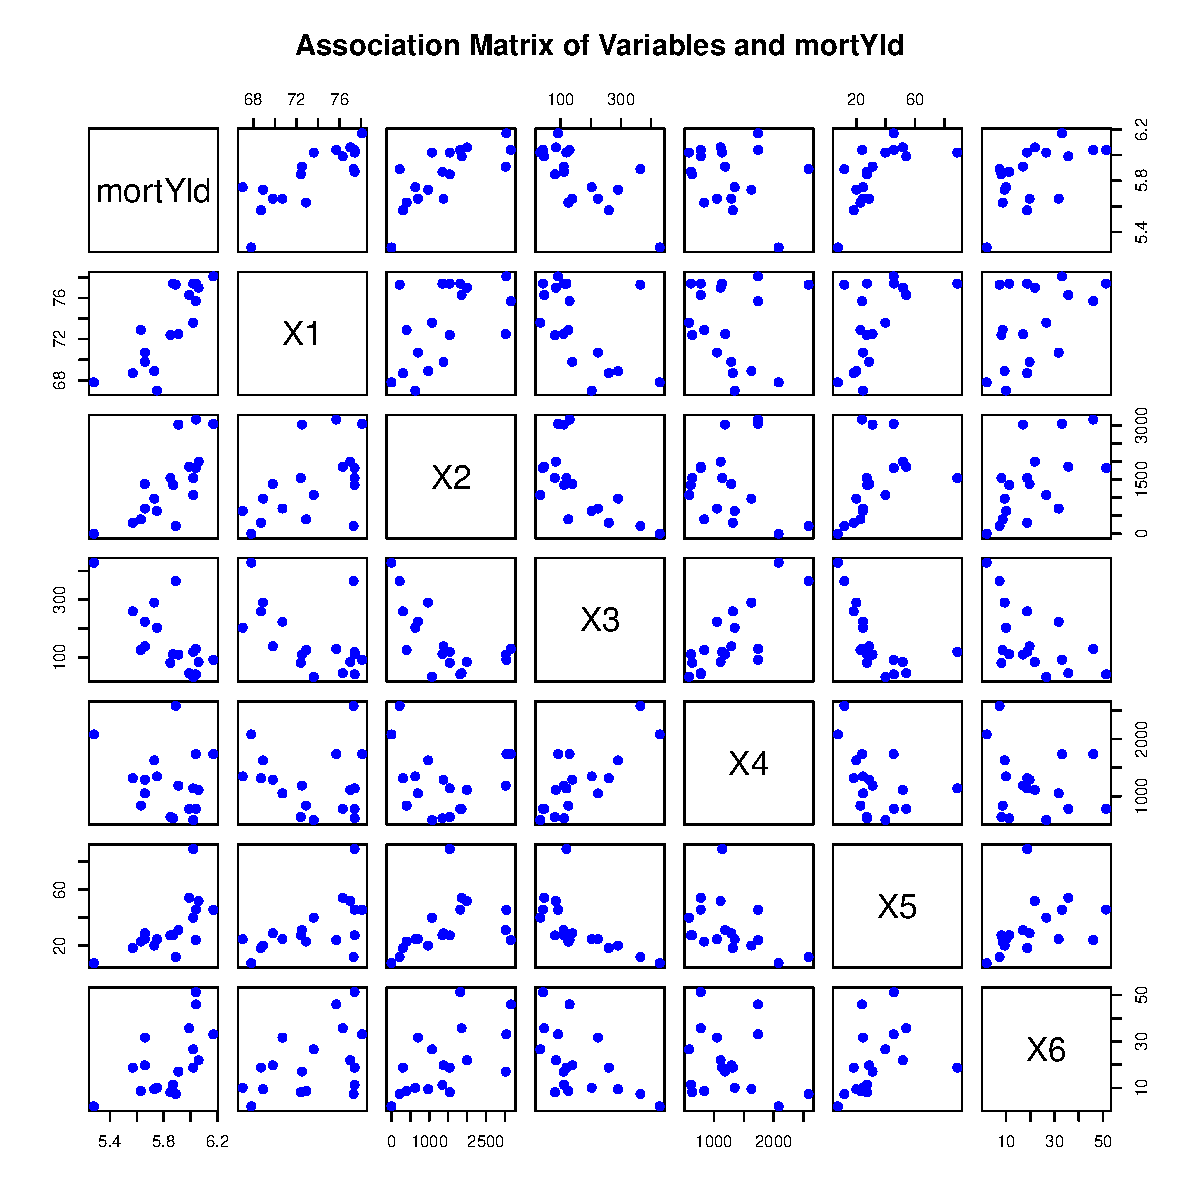
\includegraphics{Figs/unnamed-chunk-5-1.pdf} As the Loan-to-Mortgage
Ratio (X1) increases, the Mortgage Yield increases. This suggests a
positive correlation, and that higher Loan-to-Mortgage Ratios (more
borrowed money relative to the property value) are associated with
higher Mortgage Yields. Distance from Boston (X2) reveals a positive
correlation with \texttt{mortYld}. Boston represents a major financial
center with surplus capital. Regions further from Boston might have
higher Yields. Savings per New Unit Built (X3) seems to be negatively
correlated with \texttt{mortYld}. This indicates that areas with more
savings dedicated to new construction have better access to local
financing, resulting in lower Mortgage Yields. Savings per Capita (X4)'s
influence is less distinguishable but appears to be a weak negative
correlation or a random dispersion. Population Increase (X5) shows a
positive association which can be seen as a square-root relationship.
High population growth may imply higher demand for housing, increasing
Mortgage Yields due to heightened competition for available funds. We
can observe a potential outlier at the right side of the plot. The
Percentage of First Mortgages from Inter-Regional Banks (X6)'s variation
shows no clear trend. It seems like the reliance on external financing
does not significantly influence Mortgage Yields.\\
\strut \\
\textbf{To resume:}\\
- X1, X2 and X5 seem to be the most influential variables positively
correlated with Mortgage Yield.\\
- X3 is the most influential variable negatively correlated with
Mortgage Yield.\\
- X6 shows moderate positive influence on Mortgage Yield.\\
- X4 variable shows a weak relationship with Mortgage Yields.\\
\strut \\
These observations support the findings of Schaaf (1966) stating that
distance from financial centers, risk factors, and local demand for
savings contribute to Mortgage Yield variations.

\subsubsection{Correlation Analysis}\label{correlation-analysis}

\begin{minipage}{0.45\textwidth}
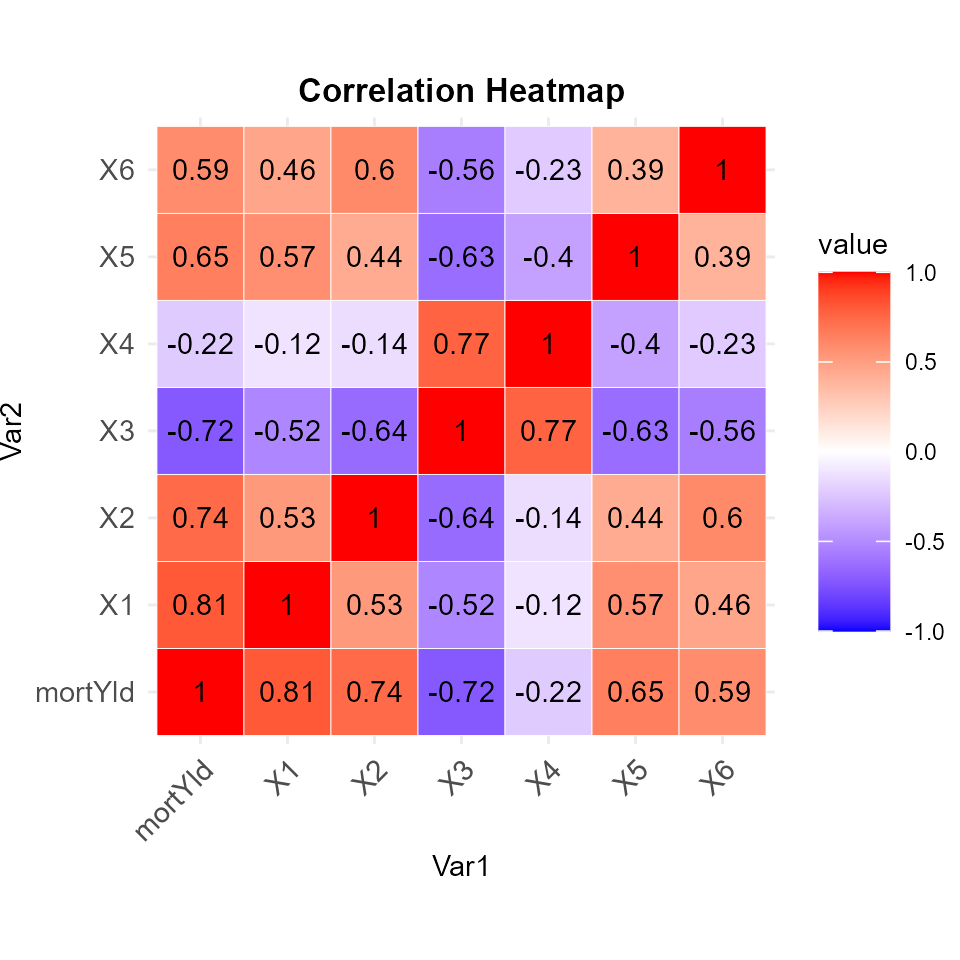
\includegraphics[width=\linewidth]{correlation_heatmap.png}
\end{minipage}
\hfill
\begin{minipage}{0.5\textwidth}
\vspace{0.5em}
\small
Now, let's take a look at the correlations between each variable and confirm our previous observations: \\
\\
- \textbf{X3} is strongly positively correlated to \textbf{X4} (0.77) and negatively to \textbf{X2} (-0.64), \textbf{X5} (-0.63), and \textbf{X6} (-0.56).\\
- \textbf{X1} and \textbf{X2} exhibit strong positive correlation with \texttt{mortYld}, while \textbf{X5} shows moderate positive correlation, and \textbf{X3} a strong negative one. \textbf{X6} shows moderate positive correlation with \texttt{mortYld} as well. \textbf{X4} shows only weak correlation with \texttt{mortYld}.\\
\\
This confirms what we saw earlier in the association matrix.
\end{minipage}

We can then think about removing one of the highly correlated
predictors, to see if multicollinearity affects the regression model.
However, these correlations only indicate if two variables are linearly
associated. Thus, a low value doesn't necessarily mean that the
variables are not correlated in another way.

\section{Model Fitting}\label{model-fitting}

In this analysis, all predictors are continuous variables and each
observation corresponds to a unique SMSA. Since the dataset contains no
grouping or categorical factors with unequal group sizes, this is a
standard multiple regression model with one observation per row.
Therefore, the design is not factorial and does not involve unbalanced
group structures. As a result, the order in which predictors are entered
into the lm() function does not influence the coefficient estimates,
F-tests, or model interpretation.

\subsection{Pairwise Simple
Regressions}\label{pairwise-simple-regressions}

\begingroup\fontsize{8}{10}\selectfont

\begin{longtable}[t]{lrr}
\caption{\label{tab:unnamed-chunk-6}Simple Linear Regressions: $R^2$ and p-values}\\
\toprule
Predictor & R\_squared & p\_value\\
\midrule
X1 & 0.654 & 0.0000\\
X2 & 0.546 & 0.0005\\
X3 & 0.517 & 0.0008\\
X4 & 0.049 & 0.3763\\
X5 & 0.419 & 0.0037\\
\addlinespace
X6 & 0.346 & 0.0103\\
\bottomrule
\end{longtable}
\endgroup{}

The table summarizes the individual linear relationships between each
predictor (X1--X6) and Mortgage Yield, assuming all other variables
remain constant, based on simple linear regression.\\
- X1 is the strongest and most significant predictor of Mortgage Yield,
explaining 65.4\% of its variance (p \textless{} 0.0001).\\
- X2 and X3 also show strong and significant linear associations
(\(R^2\) = 0.546 and 0.517, respectively with p \textless{} 0.001 and p
\textless{} 0.001).\\
- X5 and X6 show moderate yet significant associations (\(R^2\) = 0.419
and 0.346, respectively with p \textless{} 0.005 and p \textless{}
0.05).\\
- X4 doesn't exhibit a significant linear relationship with Mortgage
Yield (\(R^2\) = 0.049, p = 0.3763), suggesting it may not be a strong
individual linear predictor.\\
\strut \\
This preliminary analysis indicates that variables X1, X2, and X3 may be
the most promising candidates for predicting Mortgage Yield in a
multivariate linear model.

\subsection{Null Model vs Full Model
Comparison}\label{null-model-vs-full-model-comparison}

\begingroup\fontsize{8}{10}\selectfont

\begin{longtable}[t]{lrrrrrr}
\caption{\label{tab:unnamed-chunk-7}Comparison of Null and Full Model (ANOVA)}\\
\toprule
term & df.residual & rss & df & sumsq & statistic & p.value\\
\midrule
\cellcolor{gray!10}{mortYld \textasciitilde{} 1} & \cellcolor{gray!10}{17} & \cellcolor{gray!10}{0.8485778} & \cellcolor{gray!10}{NA} & \cellcolor{gray!10}{NA} & \cellcolor{gray!10}{NA} & \cellcolor{gray!10}{NA}\\
mortYld \textasciitilde{} X1 + X2 + X3 + X4 + X5 + X6 & 11 & 0.1098038 & 6 & 0.738774 & 12.3349 & 0.0002523\\
\bottomrule
\end{longtable}
\endgroup{}

The ANOVA comparison between the null model (intercept-only) and the
full model (including all predictors), reveals that the full model
better explains the Mortgage Yield, as shown by the significant
F-statistic and p-value (p \textless{} 0.001). This indicates that at
least one of the predictors is significantly related to Mortgage Yield,
and is useful for improving the model.

\begin{table}[!h]
\centering
\caption{\label{tab:unnamed-chunk-8}Summary of Full Linear Model}
\centering
\fontsize{8}{10}\selectfont
\begin{tabular}[t]{lrrrr}
\toprule
term & estimate & std.error & statistic & p.value\\
\midrule
(Intercept) & 4.2852 & 0.6682 & 6.4127 & 0.0000\\
X1 & 0.0203 & 0.0093 & 2.1835 & 0.0515\\
X2 & 0.0000 & 0.0000 & 0.2896 & 0.7775\\
X3 & -0.0016 & 0.0008 & -2.1029 & 0.0593\\
X4 & 0.0002 & 0.0001 & 1.7944 & 0.1002\\
\addlinespace
X5 & 0.0013 & 0.0018 & 0.7267 & 0.4826\\
X6 & 0.0002 & 0.0023 & 0.1024 & 0.9203\\
\bottomrule
\end{tabular}
\end{table}
\begin{table}[!h]
\centering
\caption{\label{tab:unnamed-chunk-9}Fit Statistics of Full Linear Model}
\centering
\fontsize{8}{10}\selectfont
\begin{tabular}[t]{rrrrrr}
\toprule
R\textsuperscript{2} & Adjusted R\textsuperscript{2} & Residual Std. Error & F-statistic & DF & p-value\\
\midrule
0.8706 & 0.8 & 0.0999 & 12.3349 & 6 & 3e-04\\
\bottomrule
\end{tabular}
\end{table}

The Full model explains \textasciitilde87\% of the variance in Mortgage
Yield, and 80\% after adjusting for the number of predictors, which
highlights a strong fit. The Residual Standard Error (?) is low, and the
overall model is statistically significant, with a very low p-value (p
\textless{} 0.001). Once again, it means that at least one term
contributes significantly to explaining the variation in
\texttt{mortYld}.\\
\strut \\
The intercept appears to be strongly significant to fit the model (p
\textless{} 0.001). On the other hand, most of the variables do not show
statistically significant individual contributions: only X1 and X3 show
weak significance (p \(\approx\) 0.05), while the other variables, X2,
X5 and X6, do not show significant individual effects. This suggests
that a reduced model may be more appropriate.\\
\strut \\
We end up with : \texttt{mortYld} = 4.2852 + 0.0203\(\times\)X1 +
0.0\(\times\)X2 - 0.0016\(\times\)X3 + 0.0002\(\times\)X4 +
0.0013\(\times\)X5 + 0.0002\(\times\)X6

\subsection{Make stepwise regression to select the best
model}\label{make-stepwise-regression-to-select-the-best-model}

\begin{minipage}{0.48\textwidth}
\centering
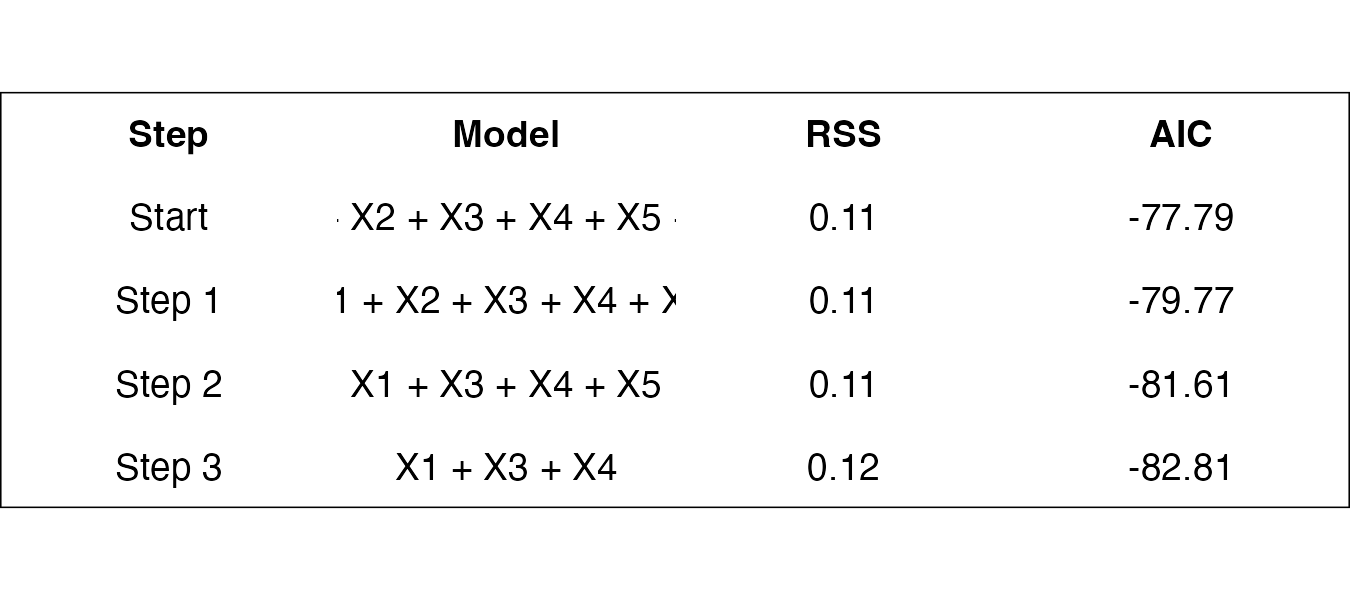
\includegraphics[width=\linewidth]{stepwise_aic_table.png}\\
\small Table 7: Stepwise AIC Steps
\end{minipage}
\hfill
\begin{minipage}{0.48\textwidth}
\centering
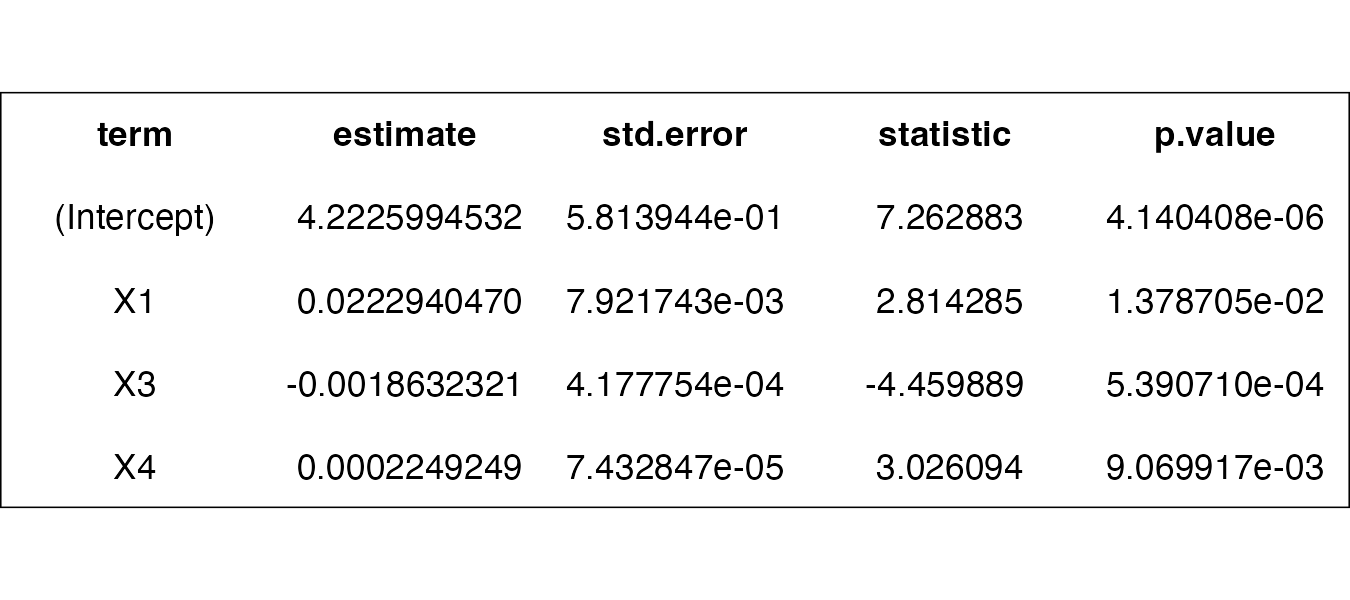
\includegraphics[width=\linewidth]{stepwise_coef_table.png}\\
\small Table 8: Coefficients of Final Stepwise Model
\end{minipage}

\addtocounter{table}{2}

\begin{table}[!h]
\centering
\caption{\label{tab:unnamed-chunk-10}Fit Statistics of Stepwise Model}
\centering
\fontsize{8}{10}\selectfont
\begin{tabular}[t]{rrrrrl}
\toprule
$R^2$ & Adjusted $R^2$ & Residual Std. Error & F-statistic & DF & p-value\\
\midrule
0.8634 & 0.8341 & 0.091 & 29.4933 & 3 & 2.62e-06\\
\bottomrule
\end{tabular}
\end{table}

The Stepwise regression process identifies X1, X3, and X4 as the most
significant predictors of Mortgage Yield, constituting the final model.

It is interesting to note that X4 appears among the 3 most significant
predictors although it shows very weak correlation in the Correlation
Matrix. Multiple regression measures the effect of each variable while
holding all others constant. As X4 has very strong correlation with X3
(0.77), holding X3 can make the unique contribution of X4 clearer.

The final Stepwise model explains approximately 83.4\% of the variance
in Mortgage Yield using only these three predictors. The AIC doesn't
increases a lot when keeping more predictors, meaning that even if these
predictors can still be statistically valid to keep, they are not so
useful to the model. Though the final model is simpler, it explains the
data just as well or better than more complex models. The Residual
Standard Error (0.091) is low, and the overall model is highly
significant (p \textless{} 0.001), indicating a good fit.\\
\strut \\
We end up with : \texttt{mortYld} = 4.223 + 0.02229\(\times\)X1 -
0.001863\(\times\)X3 + 0.0002249\(\times\)X4\\
\strut \\
Let's now try a model with 2-way interactions.

\begin{table}[!h]
\centering
\caption{\label{tab:unnamed-chunk-11}Coefficients of Interaction Model}
\centering
\fontsize{8}{10}\selectfont
\begin{tabular}[t]{lrrrr}
\toprule
term & estimate & std.error & statistic & p.value\\
\midrule
(Intercept) & 5.3710 & 2.0329 & 2.6421 & 0.0229\\
X1 & 0.0069 & 0.0266 & 0.2601 & 0.7996\\
X3 & -0.0001 & 0.0096 & -0.0108 & 0.9916\\
X4 & -0.0009 & 0.0025 & -0.3706 & 0.7180\\
X1:X3 & 0.0000 & 0.0001 & -0.1582 & 0.8772\\
\addlinespace
X1:X4 & 0.0000 & 0.0000 & 0.4641 & 0.6516\\
X3:X4 & 0.0000 & 0.0000 & -0.1046 & 0.9185\\
\bottomrule
\end{tabular}
\end{table}

\begin{table}[!h]
\centering
\caption{\label{tab:unnamed-chunk-12}Fit Statistics of Interaction Model}
\centering
\fontsize{8}{10}\selectfont
\begin{tabular}[t]{rrrrrr}
\toprule
R\textsuperscript{2} & Adjusted R\textsuperscript{2} & Residual Std. Error & F-statistic & DF & p-value\\
\midrule
0.8698 & 0.7988 & 0.1002 & 12.25 & 6 & 3e-04\\
\bottomrule
\end{tabular}
\end{table}

The 2-way Interactions model, which is more complex than the Stepwise
model, explains approximately 79.9\% of the variance in Mortgage Yield.
The Residual Standard Error (0.1002) is low, and the overall model is
highly significant (p \textless{} 0.001), indicating that at least one
of the terms has a significant influence on Mortgage Yield.

None of the variables show statistically significant individual
contributions: only the intercept appears to be moderately significant
to fit the model (p \textless{} 0.05). This suggests that a reduced
model may be more appropriate.\\
\strut \\
We end up with : \texttt{mortYld} = 5.3710 + 0.0069*X1 - 0.0001*X3 -
0.0009*X4 + 0.0*X1:X3 + 0.0*X1:X4 + 0.0*X3:X4\\
\strut \\
We decided not to include a 3-way Interactions model in our analysis.
Given the small sample size (18 observations), adding high-order
interactions would significantly reduce degrees of freedom and increase
the risk of overfitting. Moreover, 3-way interactions are often
difficult to interpret meaningfully.

\subsection{Model Comparison}\label{model-comparison}

\begingroup\fontsize{8}{10}\selectfont

\begin{longtable}[t]{lrrrrr}
\caption{\label{tab:unnamed-chunk-13}Comparison of Model Performance Metrics}\\
\toprule
Model & R2 & Adj\_R2 & AIC & Residual\_SE & F\_statistic\\
\midrule
Full Model & 0.871 & 0.800 & -24.708 & 0.100 & 12.335\\
Stepwise Model & 0.863 & 0.834 & -29.731 & 0.091 & 29.493\\
2-Way Interaction Model & 0.870 & 0.799 & -24.600 & 0.100 & 12.250\\
\bottomrule
\end{longtable}
\endgroup{}

The \textbf{Stepwise model} offers the best trade-off between simplicity
and performance: it has the lowest AIC (\textasciitilde29.7),
demonstrating the best model fit among the three. Despite having a
slightly lower R² than the Full and 2-ways Interactions model, it
achieves the highest Adjusted R². It also has the lowest Residual
Standard Error (0.091) and the highest F-statistic
(\textasciitilde29.5). This confirms the overall model significance and
parsimony.

\begin{table}[!h]
\centering
\caption{\label{tab:unnamed-chunk-14}ANOVA Comparison: Stepwise vs Interactions Model}
\centering
\fontsize{8}{10}\selectfont
\begin{tabular}[t]{lrrrrrr}
\toprule
Model & Res.Df & RSS & Df & Sum of Sq & F & Pr(>F)\\
\midrule
Stepwise model & 14 & 0.1159 & NA & NA & NA & NA\\
Interaction model & 11 & 0.1105 & 3 & 0.0055 & 0.1813 & 0.9069\\
\bottomrule
\end{tabular}
\end{table}

An ANOVA is then conducted to confirm that including 2-way Interactions
terms do not significantly improve the model fit. The test yields an
F-statistic of 0.18 and a p-value of 0.91, indicating that the
additional interaction terms do not meaningfully reduce the residual
variance.

As a result, the simpler model with only main effects (X1, X3, and X4)
truly provides the best fit, as it also offers comparable explanatory
power and better interpretability.

\section{Model assumptions and
Diagnostics}\label{model-assumptions-and-diagnostics}

\subsection{Independence evaluation}\label{independence-evaluation}

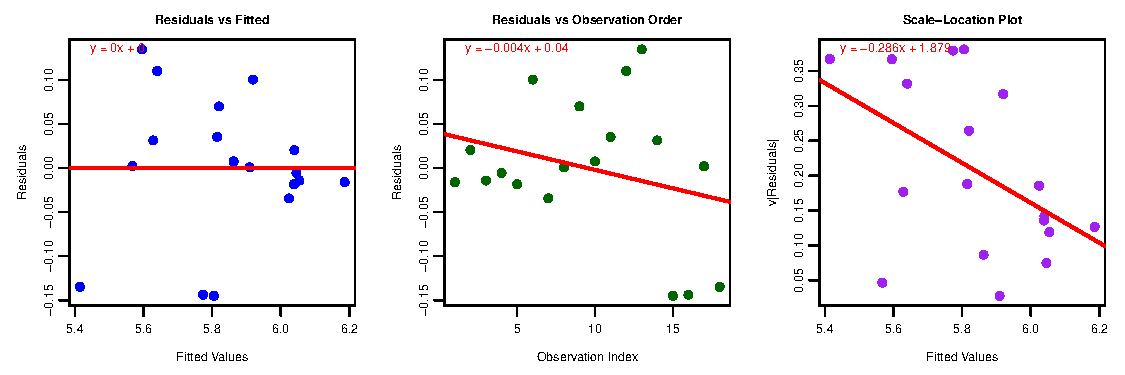
\includegraphics{Figs/unnamed-chunk-15-1.pdf}

The \texttt{Residuals\ VS\ Fitted\ Values} plot shows that the residuals
are randomly scattered around 0, with no clear pattern. This suggests
that the assumptions of linearity and constant error variance are
reasonably met. Secondly, the slightly negative but close to zero slope
(-0.286) in the \texttt{Scale-Location\ Plot} indicates that the spread
of residuals is almost constant across fitted values. This is a sign
that our model doesn't suffer from heteroscedasticity and is likely a
good fit: homoscedasticity seems therefore satisfied.

The \texttt{Residuals\ VS\ Observation\ Order} plot helps us conclude
that there is no consistent trend: the independence of residuals is
verified, as they are not correlated with the order of observations.

\subsection{Multicolinearity
diagnostic}\label{multicolinearity-diagnostic}

\begingroup\fontsize{8}{10}\selectfont

\begin{longtable}[t]{lr}
\caption{\label{tab:unnamed-chunk-16}Variance Inflation Factors (VIF)}\\
\toprule
 & vif\_values\\
\midrule
X1 & 1.886802\\
X3 & 4.550125\\
X4 & 3.348330\\
\bottomrule
\end{longtable}
\endgroup{}

As all variables have a VIF value under 5, it means that they don't
cause problematic multicollinearity in the final model and that none of
them should be eliminated. This confirms our choice of keeping X3 and
X4: even if they showed a high correlation coefficient (0.77), these
variables still provide enough unique, non-redundant information to
justify keeping them in the model.

\subsection{Normality Check}\label{normality-check}

\begin{minipage}{0.45\textwidth}
\centering
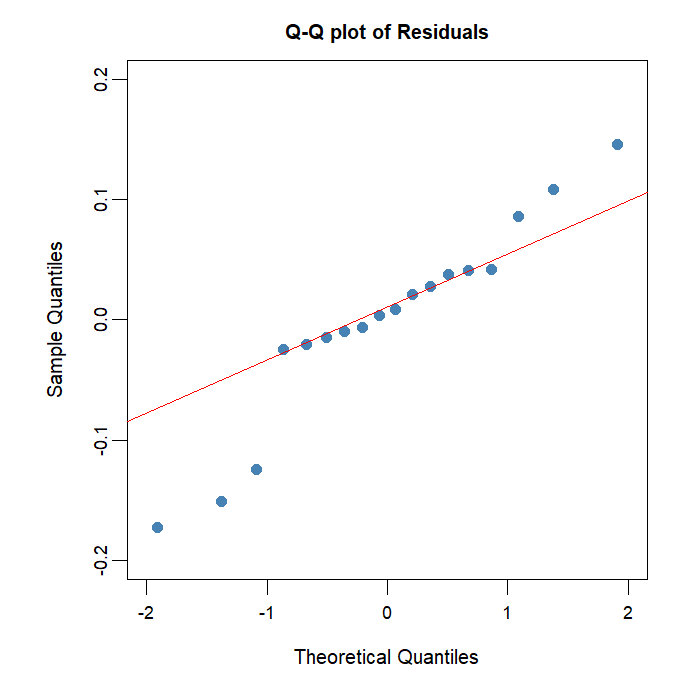
\includegraphics[width=0.85\linewidth]{qqplot_residuals.png}
\end{minipage}
\hfill
\begin{minipage}{0.5\textwidth}
\small
The \texttt{Q-Q plot of Residuals} indicates that most of the points align closely with the 45-degree line, suggesting that the residuals are approximately normally distributed. However, six points deviate at the extremes of the theoretical quantiles, which indicates the presence of potential outliers or heavy tails in the distribution. In a dataset with just 18 observations, small deviations in the Q-Q plot are usual. Outliers or deviations are common in such a small sample size and do not automatically suggest a violation of normality.
\end{minipage}

\section{Conclusions}\label{conclusions}

\hfill\break
The final estimated model is : \texttt{mortYld} = 4.223 + 0.02229*X1 -
0.001863*X3 + 0.0002249*X4\\
where X1 is the Loan-to-Mortgage Ratio, X3 is the Savings per New Unit
Built, and X4 is the Savings per Capita.

The analysis thus shows that Loan-to-Mortgage Ratio, Savings per New
Unit Built, and Savings per Capita collectively have a significant
impact on Mortgage Yield. Mortgage Yield is positively influenced by the
Loan-to-Mortgage Ratio (X1), suggesting that when the loan is higher
compared to the mortgage, lenders may see better returns on their
investment. On the other hand, Mortgage Yield is negatively impacted by
Savings per New Unit Built (X3). When there is more capital saved for
new construction, there may be less reliance on mortgages, potentially
leading to lower returns on those mortgages. Lastly, Savings per Capita
(X4) has a positive, though small, effect on the Mortgage Yield. As
individuals save more money, it may lead to a slight increase in the
return on mortgages, possibly because higher savings per capita can
signal a more financially stable environment for lenders, leading to
better mortgage performance.

While the assumptions of linear regression are generally satisfied,
there are some minor deviations. The model shows strong predictive
performance, accounting for 83.4\% of the variance in Mortgage Yield,
with homoscedasticity nearly achieved.

Future improvements could include exploring additional predictors,
testing for non-linear relationships, or refining the model to better
capture any residual heteroscedasticity.

\end{document}
